\chapter{Vorgehen zur Problemlösung}
Die Anwendung wandelt eine .dxf Grundrissdatei in .scad und .stl Dateien um, die zum Drucken benutzt werden können.
Dafür sind mehrere Zwischenschritte nötig.
\section{Einlesen des Grundrisses}
Den Beginn der Verarbeitung markiert die Grundrissdatei, in welcher sämtliche Werte, die im weiteren Verlauf des Programmes relevant werden, enthalten sind.
\subsection{Funktionsweise der Bibliothek \textit{kabeja}}
Das Einlesen der Daten eines Grundrisses, wie in Abb. 5 zu sehen, erfolgt mit der Java-Bibliothek „kabeja“. 
Diese ermöglicht es, aus .dxf-Dateien alle DXF-Objekte eines bestimmten Typs zu erhalten, deren Werte in einer Liste zu speichern und später zu verarbeiten. \\

\begin{code}[DXF File Parser]
public static ArrayList<Line> getAutocadFile(String filePath) throws ParseException {
	ArrayList<Line> vcs = new ArrayList<>();
	// Ermitteln des DXFDocuments doc
	List lst = doc.getDXFLayer("0").getDXFEntities(DXFConstants.ENTITY_TYPE_LINE);
	for (int index = 0; index < lst.size(); index++) {
		DXFLine dxfline = (DXFLine) lst.get(index);
		Line v = new Line(<Vektor des Anfangspunktes>, <Vektor des Endpunktes>);
		vcs.add(v);
	}
	return vcs;
}
\end{code}

Aus der .dxf-Datei deren Pfad der Klasse \q{DXFReader} übergeben wird, werden alle DXF-Objekte, die mit dem Typen \icode{DXFLine} übereinstimmen, in einer Liste zurückgegeben. 
Die Koordinaten der Start- und Endpunkte der DXFLines  in dieser Liste werden anschließend in eine Liste von Linien übertragen, welche unter anderem bei der Umwandlung des Graphen in die DCEL Verwendung findet.

\subsection{Funktionsweise der Benutzeroberfläche}
Die Benutzeroberfläche(GUI) setzt sich zusammen aus einem \icode{JFrame}, in dem zwei \icode{JTextField}, ein \icode{FileChooserButton}, ein \icode{StartButton} und ein \icode{ShowResultButton} platziert sind.

\begin{Bild}{Ausgangszustand der GUI (Screenshot der Verfasser)}
	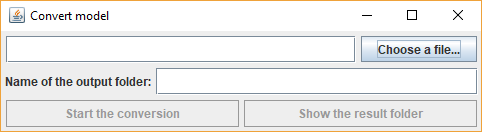
\includegraphics[width = 120mm]{Bilder/GUI/GUI_Startup}
\end{Bild}

Der Nutzer kann im Ausgangszustand über den \icode{FileChooserButton} einen \icode{JFileChooser}-Dialog öffnen, mit dem er die Datei, die er umwandeln möchte, auswählen kann.
Sobald er dann eine Datei ausgewählt hat, wird der Dateipfad zu dieser Datei zusätzlich im \icode{JTextField} angezeigt.
Alternativ zum \icode{JFileChooser}-Dialog kann der Nutzer auch direkt in das links positionierte \icode{JTextField} den Dateipfad eingeben.
Im \icode{JFileChooser} ist außerdem ein \icode{FileFilter} implementiert, der dem Nutzer lediglich .dxf-Dateien anzeigt. \\
Im \icode{JTextField} darunter gibt der Nutzer den Ordnernamen ein, in dem die umgewandelten Dateien ausgegeben werden. \\
Nachdem der Nutzer eine Datei ausgewählt und einen Namen für den Ergebnisordner eingegeben hat, wird nun der \icode{StartButton} aktiviert und er hat die Möglichkeit den Konvertierungsprozess starten.

\begin{Bild}{GUI mit aktiviertem \icode{StartButton} (Screenshot der Verfasser)}
	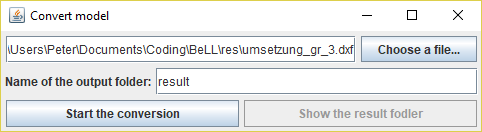
\includegraphics[width = 120mm]{Bilder/GUI/GUI_Convert_Ready}
\end{Bild}

Beim Klicken des \icode{StartButton} wird überprüft, ob das Programm die ausführbare Datei von OpenSCAD unter \icode{C:\textbackslash \textbackslash Program Files\textbackslash OpenSCAD\textbackslash } finden kann.
Diese Datei wird benötigt, um die Umwandlung der .scad-Dateien in .stl-Dateien zu ermöglichen.
Sollte diese dort nicht gefunden werden, wird der Nutzer mit einem Dialog darauf hingewiesen.

\begin{Bild}{Dialog zur Warnung des Nutzers (Screenshot der Verfasser)}
	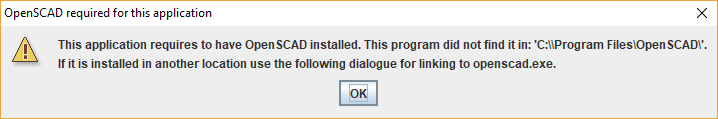
\includegraphics[width = \textwidth]{Bilder/GUI/GUI_SCAD_Error}
\end{Bild}

Anschließend hat der Nutzer die Möglichkeit, den Pfad zur ausführbaren Datei mit einem weiteren \icode{JFileChooser}-Dialog anzugeben.

\begin{Bild}{Dialog zum Verlinken der openscad.exe (Screenshot der Verfasser)}
	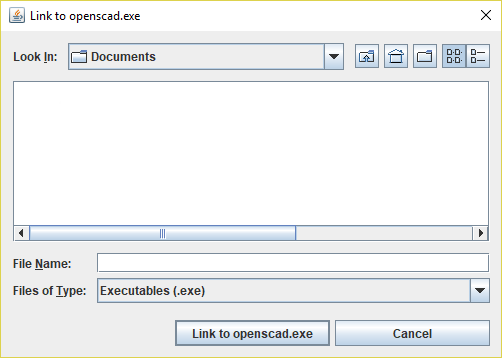
\includegraphics[width = 120mm]{Bilder/GUI/GUI_SCAD_Linking}
\end{Bild}

Sobald dieser Vorgang beendet ist, bleiben dem Nutzer nun die Möglichkeiten, den Ordner mit den Ausgabedateien anzuzeigen oder einen anderen Grundriss umzuwandeln.\\